% Paper based on the Springer LNCS proceedings template (llncs v2.25)
\documentclass[runningheads]{llncs}
%
\usepackage[T1]{fontenc}
% The template uses newtx (Times). If it is not installed, fall back to mathptmx.
\IfFileExists{newtxtext.sty}{%
  \usepackage{newtxtext}%
  \usepackage[varvw]{newtxmath}%
}{%
  \usepackage{mathptmx}%
}
\usepackage{amsmath}
\usepackage{bm}
\usepackage{graphicx}
\usepackage{booktabs}
\usepackage{tabularx}
\usepackage{xcolor}
\usepackage{tikz}
\usetikzlibrary{arrows.meta,positioning,calc}
\usepackage{pgfplots}
\pgfplotsset{compat=1.18}
\usepackage{xurl}
\usepackage[hidelinks]{hyperref}
\renewcommand\UrlFont{\color{blue}\rmfamily}
\urlstyle{rm}

\newcommand{\Pre}{\operatorname{Pre}}
\newcommand{\Rh}{\hat R}
\newcommand{\Sh}{\hat S}
\newcommand{\Lh}{\hat L}
\newcommand{\Pih}{\hat\Pi}
\newcommand{\rstar}{r^{\ast}}
\newcommand{\Slisto}{S_{\mathrm{ready}}}
\newcommand{\Smin}{S_{\min}}
\newcommand{\Carga}{\mathcal L}

\definecolor{c1}{HTML}{2A78D6}
\definecolor{c2}{HTML}{EB6834}
\definecolor{c3}{HTML}{1B8F66}
\definecolor{c4}{HTML}{6250D6}
\definecolor{cg}{HTML}{52514E}

\begin{document}
%
\title{Spaced Repetition over Prerequisite Graphs for Procedural Skills: A Model and a Simulation Study in High-School Mechanics}
%
\titlerunning{Spaced Repetition over Prerequisite Graphs for Procedural Skills}
%
\author{Gustavo S\'anchez de la Rosa \and
Marco Antonio Ramos Corchado}
%
\authorrunning{G. S\'anchez de la Rosa and M. A. Ramos Corchado}
%
\institute{Universidad Aut\'onoma del Estado de M\'exico, Toluca, M\'exico\\
\email{\{author1,author2\}@uaemex.mx}}
%
\maketitle
%
\begin{abstract}
Spaced repetition schedulers such as SM-2, half-life regression, MEMORIZE and FSRS assume that each item exercises a single, independent piece of knowledge. Solving a physics problem violates this assumption in three ways: one problem exercises several skills, a failure does not reveal which skill failed, and skills are ordered by prerequisites, so introducing topics too early or too fast wastes practice and saturates the review queue. We propose a model that extends the memory dynamics of MEMORIZE to procedural skills organized in a prerequisite graph. It combines a fractional Q-matrix that gives partial credit to direct prerequisites, an exponential forgetting model per skill, a conjunctive observation model with slip and guess that yields a Bayesian split of blame after a failure, an admission rule that introduces a topic only when its prerequisites are consolidated and the expected review load fits the session, and a submodular coverage objective that a greedy planner maximizes within $1-1/e$ of the optimum. Parameters are fitted by maximum likelihood. We evaluate the system in a Monte Carlo simulation in which the simulated students deliberately differ from the model, on a 168-subtopic graph of high-school mechanics. With equal practice time, the proposed scheduler raises the mean probability of solving a new problem 30 days after the course by 0.090 and 0.047 over an SM-2 baseline in two scenarios, mostly by covering more topics. The advantage disappears on a coarse 15-unit graph and turns into a loss when the graph contains false dependencies.

\keywords{Spaced repetition \and Procedural skills \and Prerequisite graphs \and Student modeling \and Submodular optimization.}
\end{abstract}

%=====================================================================
\section{Introduction}
%=====================================================================

Distributing practice over time improves long-term retention compared with massed practice, and the benefit grows when each session requires active retrieval \cite{cepeda2006,kang2016}. Computational spaced repetition turns this finding into a scheduling problem: decide when each item should be reviewed so that it is not forgotten. Algorithms range from heuristic interval rules such as SM-2 \cite{wozniak1990} to models fitted from data, such as half-life regression (HLR) \cite{settles2016} and FSRS \cite{ye2022,su2023}, and to stochastic optimal control, where MEMORIZE derives that the optimal review intensity is proportional to the probability of having forgotten \cite{tabibian2019}.

All of these methods treat items as independent units of declarative knowledge, such as words or flashcards. Choffin et al.\ observe that adaptive spacing algorithms had, to their knowledge, only considered single-component items \cite{choffin2021}. Solving physics problems, a central task in high-school science and in university admission exams, breaks this assumption in three ways:

\begin{enumerate}
\item \emph{Credit.} A projectile problem requires vector decomposition, uniformly accelerated motion and the independence of horizontal and vertical motion. Each attempt is evidence about several skills.
\item \emph{Blame.} A wrong answer does not say which of those skills failed.
\item \emph{Order and saturation.} A topic introduced before its prerequisites are firm is learned poorly, and every new topic adds future reviews. Introducing material faster than it can be reviewed collapses net learning \cite{reddy2016}.
\end{enumerate}

This paper makes four contributions. (i) A memory and observation model for multi-skill problems that extends the jump dynamics of MEMORIZE with a fractional Q-matrix and a Bayesian blame rule (Sect.~\ref{sec:model}). (ii) A daily planner with an admission rule that combines a knowledge-space outer fringe with an explicit review-load constraint, and a submodular coverage objective with an approximation guarantee (Sect.~\ref{sec:planner}). (iii) A simulation study, with a deliberately misspecified simulated student, on prerequisite graphs of high-school mechanics at two levels of granularity (Sects.~\ref{sec:sim}--\ref{sec:results}). (iv) Evidence about \emph{when} such a model helps: on a fine-grained graph with a scarce practice budget and faithful dependencies, and not otherwise.

%=====================================================================
\section{Related Work}
%=====================================================================

\paragraph{Spaced repetition schedulers.} SM-2 multiplies the previous interval by a per-card ease factor adjusted by self-rated recall \cite{wozniak1990}. HLR learns the half-life of each item from the review history and features of the item \cite{settles2016}. MEMORIZE models reviews as a point process and recall $m(t)$ as a jump process, $dm=-n\,m\,dt+(1-m)\,dN$, in which the forgetting rate $n$ is multiplied by $(1-\alpha)$ after a success and by $(1+\beta)$ after a failure; minimizing a quadratic loss gives an optimal intensity $u^\ast(t)\propto 1-m(t)$ \cite{tabibian2019}, later validated in a large randomized experiment \cite{upadhyay2021}. FSRS tracks difficulty, stability and retrievability per card and chooses intervals by solving a stochastic shortest-path problem \cite{ye2022,su2023}. Reddy et al.\ model the Leitner system as a queueing network and show a phase transition: above a maximum rate of introduction of new items, items pile up in the first boxes \cite{reddy2016}. All of these methods assume independent, single-skill items.

\paragraph{Multi-skill items.} DAS3H extends additive factor models with per-skill forgetting windows, so that the prediction for an item combines the histories of all its skills \cite{choffin2019}. Choffin et al.\ extend adaptive spacing heuristics to multi-skill items with greedy subset selection \cite{choffin2021}; this is the closest antecedent to our planner, but it uses neither prerequisites nor load control. Math Academy describes a proprietary scheme, \emph{fractional implicit repetition}, in which credit for an advanced topic flows fractionally to the topics it uses \cite{skycak2023}; to our knowledge it has no published model or controlled evaluation.

\paragraph{Student models and knowledge structure.} Bayesian knowledge tracing introduced slip and guess parameters for noisy observations of a latent skill \cite{corbett1994}. The Q-matrix maps items to required skills \cite{tatsuoka1983}; conjunctive cognitive diagnosis models such as DINA and G-DINA assume that a correct answer requires all of them \cite{junker2001,delatorre2011}, whereas AFM and PFA add skill contributions \cite{cen2006,pavlik2009}. The KLI framework stresses that the granularity of knowledge components is an empirical question \cite{koedinger2012}. Knowledge space theory defines the \emph{outer fringe} of a knowledge state as the items whose prerequisites are mastered \cite{doignon1985}. Hunziker et al.\ teach several concepts to a forgetful learner with submodular objectives and approximation guarantees \cite{hunziker2019}.

\paragraph{Spacing in procedural domains.} Skill decay with disuse is well documented \cite{arthur1998}, and interleaved and spaced practice improves mathematics learning \cite{rohrer2015}, although classroom evidence for procedures is less consistent than for facts \cite{barzagar2019}. In physics, spaced use of a web tool was associated with higher exam scores in a university thermodynamics course \cite{voice2020}, with a fixed, non-adaptive schedule.

%=====================================================================
\section{Model}
\label{sec:model}
%=====================================================================

Let $G=(\mathcal K,E)$ be a directed acyclic graph whose nodes are skills (subtopics) and whose edges $p\to k$ mean that $p$ is a prerequisite of $k$; $\Pre(k)$ denotes the direct prerequisites of $k$ and $t$ is time in days. A problem \emph{of type} $j$ is generated from a parametric template whose main skill is $j$. For each introduced skill the state stores an estimated stability $\Sh_k$ and the effective time of its last review $\Lh_k$.

\paragraph{Fractional Q-matrix.} A problem of type $j$ fully exercises $j$ and partially exercises its direct prerequisites:
\begin{equation}
w_{jk}=\begin{cases}1 & k=j,\\ w_{\mathrm{pre}} & k\in\Pre(j),\\ 0 & \text{otherwise,}\end{cases}
\qquad Q(j)=\{j\}\cup\Pre(j),
\label{eq:w}
\end{equation}
with $w_{\mathrm{pre}}=0.5$ as an initial assumption that can later be estimated per edge.

\paragraph{Memory.} Following MEMORIZE, estimated recall decays exponentially, with stability $\Sh_k=1/\hat n_k$ (days until recall falls to $e^{-1}$):
\begin{equation}
\Rh_k(t)=\exp\bigl(-(t-\Lh_k)/\Sh_k\bigr).
\label{eq:mem}
\end{equation}

\paragraph{Observation.} Solving requires retrieving every component (a conjunctive model, as in DINA), with slip $s$ and guess $g$ as in BKT:
\begin{equation}
\Pih_j(t)=\prod_{k\in Q(j)}\Rh_k(t)^{\,w_{jk}},\qquad
\hat P_j(t)=(1-s)\,\Pih_j(t)+g\,\bigl(1-\Pih_j(t)\bigr).
\label{eq:obs}
\end{equation}
The weight in the exponent makes a half-forgotten prerequisite less harmful than a half-forgotten main skill: with $\Rh=0.6$, it is retrieved with probability $0.6^{0.5}\approx0.77$.

\paragraph{Update after a success.} Stability grows in proportion to what had been forgotten, in line with the retrieval-effort hypothesis \cite{pyc2009}:
\begin{equation}
\Sh_k\leftarrow\Sh_k\,\bigl[1+w_{jk}\,G\,(1-\Rh_k)\bigr],\qquad k\in Q(j).
\label{eq:success}
\end{equation}
The gain vanishes when $\Rh_k=1$, so massed practice right after instruction does not build long-term memory. If every review happens at $\Rh=\rstar$, stability is multiplied by $1+G(1-\rstar)$ and intervals grow geometrically.

\paragraph{Recall jump.} After any attempt the student sees the worked solution, so recall rises. This is the MEMORIZE jump $dm=(1-m)\,dN$, weighted by $w_{jk}$:
\begin{equation}
\Rh_k^{+}=\Rh_k+w_{jk}(1-\Rh_k),\qquad \Lh_k\leftarrow t+\Sh_k^{+}\ln\Rh_k^{+},
\label{eq:jump}
\end{equation}
where the second expression chooses the effective review time that makes \eqref{eq:mem}, with the new stability, return exactly $\Rh_k^{+}$.

\paragraph{Blame after a failure.} Which component failed is not observed. By Bayes' rule, the probability that component $k$ was not retrieved given a failure is
\begin{equation}
b_k=\frac{\bigl(1-\Rh_k^{\,w_{jk}}\bigr)(1-g)}{\Pih_j\,s+\bigl(1-\Pih_j\bigr)(1-g)},
\label{eq:blame}
\end{equation}
which reduces to $b_k=(1-\Rh_k^{\,w_{jk}})/(1-\Pih_j)$ when $s=g=0$; the simulations below use this simple form. Blame concentrates on the component most likely to have failed, and the full form shrinks it when $\Pih_j\approx1$, because such a failure is better explained by a slip.

\paragraph{Update after a failure.} Each component loses stability in proportion to its blame, with a floor $\Smin$, and the jump \eqref{eq:jump} is then applied:
\begin{equation}
\Sh_k\leftarrow\max\bigl(\Smin,\ \Sh_k(1-\lambda\,b_k)\bigr),\qquad k\in Q(j).
\label{eq:fail}
\end{equation}
Stability is updated at most once per skill per session: later attempts on the same day, and attempts on a skill introduced that day, only apply the jump.

\paragraph{Parameter estimation.} Given the event history, the state before each attempt is a deterministic function of $\bm\phi=(\Sh_0,G,\lambda)$, where $\Sh_0$ is the stability of a newly introduced skill. The prediction $\hat P_{in}(\bm\phi)$ for attempt $n$ of student $i$ is therefore known, and we minimize the Bernoulli negative log-likelihood
\begin{equation}
\mathrm{NLL}(\bm\phi)=-\sum_{i,n}\Bigl[y_{in}\ln\hat P_{in}(\bm\phi)+(1-y_{in})\ln\bigl(1-\hat P_{in}(\bm\phi)\bigr)\Bigr]
\label{eq:nll}
\end{equation}
with Nelder--Mead on $(\ln\Sh_0,\ln G,\operatorname{logit}\lambda)$. For identifiability, the calibration data should come from a pilot with varied review intervals rather than from the final policy.

%=====================================================================
\section{Daily Planner}
\label{sec:planner}
%=====================================================================

\paragraph{Review load.} A skill is reviewed roughly every $\Sh_k\ln(1/\rstar)$ days, where $\rstar$ is the target retention. The expected load, in problems per session, is
\begin{equation}
\Carga=\sum_{k\ \text{introduced}}\min\Bigl(1,\ \frac{f}{\Sh_k\ln(1/\rstar)}\Bigr),
\label{eq:load}
\end{equation}
where $f$ converts days into sessions ($f=7/5$ for five sessions per week). As $\Sh_k$ grows, a mature skill's load tends to zero and frees room for new topics.

\paragraph{Admission.} With $U$ problems per session and $m$ skills already admitted today, a skill $k$ that has not been introduced is admissible if
\begin{equation}
\forall p\in\Pre(k):\ \Sh_p\ge\Slisto\ \text{and}\ \Rh_p(t)\ge\rstar,
\qquad\text{and}\qquad
\Carga+m+1\le\rho\,U.
\label{eq:admit}
\end{equation}
The first condition is the outer fringe of knowledge space theory \cite{doignon1985} with ``mastered'' replaced by ``stable in memory''; the second turns the saturation result of Reddy et al.\ \cite{reddy2016} into an explicit constraint, with $\rho<1$ reserving room for reviews.

\paragraph{Submodular coverage.} Let $D=\{k:\Rh_k<\rstar\}$ be the overdue skills and $\pi_k=1-\Rh_k$ their priority, which has the form of the MEMORIZE intensity $u^\ast\propto1-m$. The planner selects a set $A$ of problem types maximizing the covered overdue mass
\begin{equation}
V(A)=\sum_{k\in D}\pi_k\Bigl[1-\prod_{j\in A}(1-w_{jk})\Bigr],
\label{eq:cover}
\end{equation}
among types whose other components satisfy $\Rh\ge r_{\min}$, so that a problem is not chosen when a forgotten prerequisite would make it unsolvable. $V$ is a weighted coverage function, hence monotone and submodular, and the greedy algorithm that adds the type with the largest marginal gain $\Delta(j\mid A)=\sum_{k\in D}\pi_k\,w_{jk}\prod_{j'\in A}(1-w_{j'k})$ achieves at least $1-1/e$ of the optimum under a cardinality constraint \cite{nemhauser1978}. The objective favors integrative problems that review several overdue skills at once.

\paragraph{Session.} The plan for each day is built in three phases: (1) greedy coverage of overdue skills; (2) admission of up to $m_{\max}$ new skills by \eqref{eq:admit}, each of which uses $n_{\mathrm{intro}}$ slots for a worked example and initial practice; (3) early reviews of the skills with the lowest recall if slots remain. Fig.~\ref{fig:loop} summarizes the cycle.

\begin{figure}[t]
\centering
\resizebox{\textwidth}{!}{%
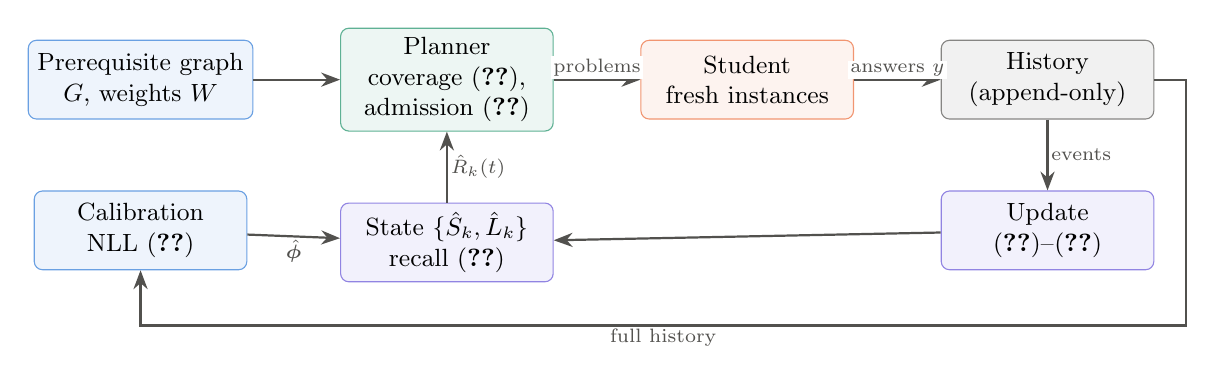
\begin{tikzpicture}[font=\small,
  box/.style={draw=#1!70, fill=#1!8, rounded corners=3pt, minimum height=10mm, minimum width=27mm, align=center},
  ar/.style={-{Stealth[length=2.4mm]}, thick, cg},
  lb/.style={font=\scriptsize, text=cg, fill=white, inner sep=1pt}]
\node[box=c1] (g) {Prerequisite graph\\$G$, weights $W$};
\node[box=c3, right=11mm of g] (p) {Planner\\coverage \eqref{eq:cover},\\admission \eqref{eq:admit}};
\node[box=c2, right=11mm of p] (s) {Student\\fresh instances};
\node[box=cg, right=11mm of s] (h) {History\\(append-only)};
\node[box=c4, below=9mm of p] (st) {State $\{\Sh_k,\Lh_k\}$\\recall \eqref{eq:mem}};
\node[box=c4, below=9mm of h] (u) {Update\\\eqref{eq:success}--\eqref{eq:fail}};
\node[box=c1, below=9mm of g] (c) {Calibration\\NLL \eqref{eq:nll}};
\draw[ar] (g) -- (p);
\draw[ar] (p) -- node[lb,above]{problems} (s);
\draw[ar] (s) -- node[lb,above]{answers $y$} (h);
\draw[ar] (h) -- node[lb,right]{events} (u);
\draw[ar] (u) -- (st);
\draw[ar] (st) -- node[lb,right]{$\Rh_k(t)$} (p);
\draw[ar] (h.east) -- ++(4mm,0) |- node[lb,below,pos=0.75]{full history} ($(c.south)+(0,-7mm)$) -- (c.south);
\draw[ar] (c) -- node[lb,below]{$\hat{\bm\phi}$} (st);
\end{tikzpicture}}
\Description{Block diagram. The prerequisite graph feeds the planner, which sends problems to the student. Answers are appended to the history, which drives the update of the state; the state feeds recall estimates back to the planner. The full history also feeds a calibration step whose parameters feed the state.}
\caption{Daily cycle of the system. The state is always a replay of the append-only history under the current parameters, so the model can be recalibrated without losing information.}
\label{fig:loop}
\end{figure}

%=====================================================================
\section{Simulation Study}
\label{sec:sim}
%=====================================================================

Evaluating the planner with the same model that generates the data would guarantee success by construction. The simulator therefore separates the \emph{truth} (how the simulated student learns and forgets, never seen by the planner) from the \emph{model} of Sects.~\ref{sec:model}--\ref{sec:planner}, and misspecifies the latter on purpose (Table~\ref{tab:truth}).

\begin{table}[t]
\centering
\caption{Deliberate differences between the simulated student and the planner's model.}
\label{tab:truth}
\setlength{\tabcolsep}{4pt}
\begin{tabularx}{\textwidth}{@{}l>{\raggedright\arraybackslash}X>{\raggedright\arraybackslash}X@{}}
\toprule
& Truth (simulated student) & Model (planner) \\
\midrule
Forgetting & power law $R=(1+F\Delta t/S)^{C}$ & exponential \eqref{eq:mem} \\
Gain & FSRS-like $\gamma S^{-b}(e^{c(1-R)}-1)$ & $G(1-\Rh)$ \eqref{eq:success} \\
Failure & lapse only in components not retrieved & blame split \eqref{eq:blame} \\
Weak bases & depends on scenario (A or B) & admission gate only \\
Heterogeneity & latent ability $\theta_i\sim N(0,0.35^2)$ & none \\
\bottomrule
\end{tabularx}
\end{table}

\paragraph{Simulated student.} Student $i$ has latent ability $\theta_i$. Let $\tilde d_k$ be the depth of skill $k$ in the graph, rescaled so that the deepest skill has depth 6 in the subtopic graphs. Initial stability is $S^0_{ik}=S_0e^{\theta_i-\delta\tilde d_k}$ and the gain scale is $\gamma_{ik}=e^{a+0.5\theta_i-0.1\tilde d_k}$. True recall follows the FSRS power law $R_k(t)=(1+F\,(t-L_k)/S_k)^{C}$ with $F=19/81$ and $C=-0.5$, so that $S$ is the number of days until recall falls to 0.9. When a skill is introduced, its stability is $S^0_{ik}\prod_{p\in\Pre(k)}r_p^{\,w_{\mathrm{pre}}}$ (floored at $\Smin$), where $r_p=R_p(t)$ in scenario~A and $r_p=R_p(t)(1-e^{-S_p/\kappa})$ in scenario~B. In an attempt, each component is retrieved with probability $R_k^{\,w_{jk}}$; the answer is correct with probability $1-s$ if all components were retrieved and $g$ otherwise. Memory changes according to what was \emph{actually} retrieved: a retrieved component gains $S_k\leftarrow S_k[1+w_{jk}c_k\gamma_{ik}S_k^{-b}(e^{c(1-R_k)}-1)]$ and a non-retrieved one lapses, $S_k\leftarrow\max(\Smin,S_k(1-\ell w_{jk}))$. In scenario~B, $c_k=\prod_{p\in\Pre(k)}(1-e^{-S_p/\kappa})^{w_{\mathrm{pre}}}$, so that reviews of a skill consolidate less while its prerequisites are fragile; in scenario~A, $c_k=1$. We use $S_0=0.6$ days, $\delta=0.15$, $a=\ln4$, $b=0.15$, $c=2$, $\ell=0.6$, $\kappa=4$ days, $s=0.05$, $g=0.02$ and $\Smin=0.2$ days.

\paragraph{Domain.} We use a prerequisite graph of high-school classical mechanics at two levels of granularity. The \emph{unit} graph has 15 units in seven areas (mathematical foundations, kinematics, dynamics, momentum, work and energy, systems, rotation) and 26 edges, with maximum depth 8. The \emph{subtopic} graph has 168 subtopics of those units (for example, ``horizontal range'' or ``kinetic friction force'') and 279 hand-annotated dependencies, with maximum depth 20. As a structural control, the \emph{linear} variant replaces explicit dependencies with chains: each unit becomes a sequence of its subtopics, and each edge between units links the last subtopic of the source to the first of the target (maximum depth 103).

\paragraph{Policies.} \emph{Proposed}, with $\rstar=0.7$, $r_{\min}=0.6$, $\Slisto=7$ days, $\rho=0.8$, $w_{\mathrm{pre}}=0.5$; also with $\rstar=0.9$, and four ablations: no prerequisite credit ($w_{\mathrm{pre}}=0$ in the model), no Bayesian blame ($b_k=1$), no load control, and no prerequisite gate. \emph{Anki SM-2}: one card per topic, introduced in textbook order up to $m_{\max}$ per day, intervals $1$, $6$, $I\cdot E$ and initial ease $E=2.5$. \emph{Blocked textbook}: topics in textbook order without review. \emph{Textbook with cumulative review}: the same, but 2 of the $U$ problems of each session are drawn at random from earlier topics. All policies receive the same number of problems per session.

\paragraph{Protocol and metric.} The course lasts 12 weeks with five sessions per week (60 sessions). The unit graph uses $U=6$, $n_{\mathrm{intro}}=3$, $m_{\max}=1$; the subtopic graphs use $U=10$, $n_{\mathrm{intro}}=2$, $m_{\max}=3$. The main metric is the mean, over \emph{all} skills of the graph, of the probability that the student solves a new problem of each skill 30 days after the last session, without intermediate practice. An unintroduced skill counts as $g=0.02$, so the metric rewards both retention and coverage. Each policy is applied to the same 300 simulated students and differences are paired by student. The parameters $\bm\phi$ are estimated per scenario from a simulated pilot with 100 different students, in which topics are introduced in textbook order and reviewed at random times.

%=====================================================================
\section{Results}
\label{sec:results}
%=====================================================================

\paragraph{Unit graph: ample budget.} With 15 units and 60 sessions there are four sessions per topic, and every policy introduces the whole syllabus. Any spaced policy beats the blocked textbook by 0.28--0.29, but the proposed scheduler (0.743 in scenario~A, 0.714 in~B) does not beat Anki SM-2 (0.749 and 0.722); the prerequisite gate costs 0.009--0.011 because it delays introductions in a deep graph. A small advantage appears only with a scarce budget ($U=4$): 0.731 versus 0.714 in~A and 0.695 versus 0.681 in~B. The pilot estimates were $\Sh_0=5.23$, $G=6.07$, $\lambda=0.09$ in~A.

\paragraph{Subtopic graph: scarce budget.} With 168 subtopics no adaptive policy introduces the whole syllabus, and the picture changes (Table~\ref{tab:sub}, Fig.~\ref{fig:bars}). The pilot estimates were $\Sh_0=8.2$, $G=7.2$, $\lambda=0.13$ in~A. The proposed scheduler beats Anki by $+0.090$ in~A and $+0.047$ in~B, and the advantage holds for $U\in\{6,10,14\}$. The mechanism is coverage: Anki accumulates overdue reviews and stops introducing topics (71 versus 106 in~A, 63 versus 79 in~B). Prerequisite credit contributes $+0.014$ in~A, because an advanced problem reviews several subtopics when slots are scarce; the gate contributes $+0.015$ in~B, where learning on fragile bases causes lasting harm; Bayesian blame contributes only $+0.002$ to $+0.004$. Removing load control \emph{improves} the metric by $+0.027$ at the cost of more topics with less retention, so in this metric the load constraint is conservative.

\begin{table}[t]
\centering
\caption{Subtopic graph (168 nodes, $U=10$). Delayed test (mean per student), paired difference with respect to the proposed scheduler, topics introduced, and number of subtopics with $P\ge0.8$. 95\% confidence intervals of the differences are about $\pm0.002$.}
\label{tab:sub}
\setlength{\tabcolsep}{3.2pt}
\begin{tabular}{@{}lcccccccc@{}}
\toprule
& \multicolumn{4}{c}{A: mild weak-base effect} & \multicolumn{4}{c}{B: persistent effect} \\
\cmidrule(lr){2-5}\cmidrule(lr){6-9}
Policy & Test & $\Delta$ & Topics & $P\!\ge\!0.8$ & Test & $\Delta$ & Topics & $P\!\ge\!0.8$ \\
\midrule
Proposed ($\rstar=0.7$) & 0.370 & --- & 106 & 5.5 & 0.285 & --- & 79 & 7.1 \\
Proposed ($\rstar=0.9$) & 0.239 & $-0.131$ & 56 & 12.6 & 0.189 & $-0.097$ & 42 & 13.1 \\
\quad no prerequisite credit & 0.355 & $-0.014$ & 98 & 8.2 & 0.282 & $-0.003$ & 74 & 9.6 \\
\quad no Bayesian blame & 0.366 & $-0.004$ & 103 & 6.3 & 0.283 & $-0.002$ & 78 & 7.3 \\
\quad no load control & 0.397 & $+0.027$ & 134 & 2.3 & 0.312 & $+0.026$ & 101 & 3.2 \\
\quad no prerequisite gate & 0.372 & $+0.002$ & 108 & 4.9 & 0.270 & $-0.015$ & 79 & 6.5 \\
Anki SM-2 & 0.280 & $-0.090$ & 71 & 11.0 & 0.239 & $-0.047$ & 63 & 8.5 \\
Textbook + review & 0.275 & $-0.095$ & 168 & 1.6 & 0.144 & $-0.142$ & 168 & 1.1 \\
Blocked textbook & 0.167 & $-0.203$ & 168 & 0.0 & 0.078 & $-0.207$ & 168 & 0.0 \\
\bottomrule
\end{tabular}
\end{table}

\begin{figure}[t]
\centering
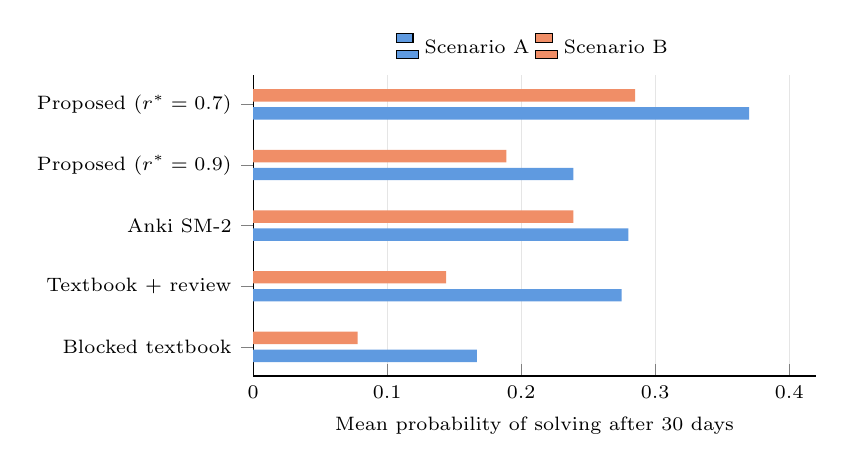
\begin{tikzpicture}
\begin{axis}[
  xbar, width=0.72\textwidth, height=5.4cm, bar width=4.5pt,
  enlarge y limits=0.12, xmin=0, xmax=0.42,
  xlabel={Mean probability of solving after 30 days},
  symbolic y coords={bt,tr,anki,p9,p7},
  yticklabels={Blocked textbook,Textbook + review,Anki SM-2,Proposed ($r^*=0.9$),Proposed ($r^*=0.7$)},
  ytick=data, tick label style={font=\scriptsize}, label style={font=\scriptsize},
  x tick label style={/pgf/number format/fixed},
  legend style={at={(0.5,1.02)},anchor=south,legend columns=2,font=\scriptsize,draw=none},
  axis lines*=left, xmajorgrids, grid style={gray!20}]
\addplot[fill=c1!75, draw=none] coordinates {(0.167,bt) (0.275,tr) (0.280,anki) (0.239,p9) (0.370,p7)};
\addplot[fill=c2!75, draw=none] coordinates {(0.078,bt) (0.144,tr) (0.239,anki) (0.189,p9) (0.285,p7)};
\legend{Scenario A, Scenario B}
\end{axis}
\end{tikzpicture}
\Description{Horizontal bar chart of the delayed test by policy and scenario on the subtopic graph. The proposed scheduler with target retention 0.7 has the longest bars in both scenarios (0.370 and 0.285), followed by Anki SM-2 (0.280 and 0.239); the blocked textbook has the shortest bars (0.167 and 0.078).}
\caption{Delayed test on the subtopic graph by policy and scenario (data from Table~\ref{tab:sub}).}
\label{fig:bars}
\end{figure}

\paragraph{Coverage versus retention.} The metric mixes two quantities. Discounting the contribution $g$ of unintroduced topics, the mean probability \emph{over introduced topics} is about 0.58 for the proposed scheduler, 0.64 for Anki and 0.68 for the proposed scheduler with $\rstar=0.9$ in~A (0.58 and 0.60 for the first two in~B). The $P\ge0.8$ column tells the same story: Anki and the $\rstar=0.9$ variant leave more subtopics ``mastered''. The proposed scheduler with $\rstar=0.7$ wins because it covers more topics with somewhat lower retention per topic. Lowering $\rstar$ further improves the metric (0.403 with $\rstar=0.5$ in~A), whereas $\rstar\ge0.9$ degrades it sharply: reviewing at $\Rh\approx0.9$ yields little gain under the true dynamics, and the estimated load \eqref{eq:load} inflates and blocks admission. The choice of $\rstar$ is therefore a pedagogical decision about this frontier, not a technical detail.

\paragraph{Graph structure matters.} On the linear variant, the advantage over Anki in scenario~A shrinks from $+0.090$ to $+0.012$ (0.298 versus 0.286). In scenario~B the proposed scheduler falls to 0.124, below Anki's 0.238: with 103 levels only one topic is admissible at a time, and the gate leaves the system with 28 topics for the whole course. Anki, which ignores the graph, is unaffected. A graph with false dependencies penalizes precisely the scheduler that respects it. One caveat is that depth rescaling differs between the two graphs, so the comparison also changes the relative difficulty of topics in the truth.

\paragraph{Calibration.} Out of sample, on attempts generated by the proposed policy, the exponential model reaches an AUC of 0.67 and a Brier score of 0.17--0.18 on the subtopic graph (AUC 0.66--0.70 on the unit graph), and it overestimates success in the middle range. This is expected, since the truth uses power-law forgetting and hidden lapses. The planner works reasonably well despite the misspecification, and calibration is the natural diagnostic to detect it with real data.

%=====================================================================
\section{Discussion and Limitations}
%=====================================================================

Across all conditions, the largest and most robust effect is spacing versus blocked instruction ($+0.20$ to $+0.29$). Among spaced policies, the proposed model helps only when two conditions hold: the graph is fine-grained relative to the practice budget, and its dependencies are real. Its finer components (Bayesian blame, prerequisite credit, gate) have small, scenario-dependent effects; the dominant mechanism is that load-aware admission keeps introducing topics where a flashcard scheduler stalls. These findings echo the KLI warning that granularity is an empirical matter \cite{koedinger2012}, and they make the validation of the prerequisite graph as important as the review rule.

The study has clear limitations. (i) The truth is itself a model: the results indicate which components \emph{could} matter and under which assumptions, not how much a classroom would gain. (ii) The value $\rstar=0.7$ was chosen after a preliminary sweep that used the truth; it should be fixed by a procedure that does not, for instance optimizing it in simulation under the model fitted to pilot data. (iii) The metric favors coverage, and a low $\rstar$ implies more failures during practice, with possible motivational costs that are not modeled. (iv) The 279 subtopic dependencies are a hand-annotated draft pending validation by teachers. (v) The model fixes $s$ and $g$, uses the simple blame rule, and has no per-student or per-skill effects; in the linear variant of scenario~B the estimate $\hat\lambda\approx0$ suggests identifiability problems. (vi) Interleaving, fatigue, dropout and variation across instances of the same problem type are not modeled \cite{rohrer2015}.

%=====================================================================
\section{Conclusion and Future Work}
%=====================================================================

We extended the memory dynamics of MEMORIZE to procedural skills linked by prerequisites, with fractional credit, Bayesian blame, load-aware admission and a submodular planner with a $1-1/e$ guarantee. In simulation on high-school mechanics, the scheduler outperforms an SM-2 baseline on a fine-grained graph with a scarce budget, mostly through coverage, and it is harmed by false dependencies. A web prototype implementing the model on 13 kinematics subtopics with 33 parametric templates already exists. Next steps are a calibration pilot with random review intervals to estimate the parameters, test the fractional Q-matrix against independent skills, and compare exponential and power-law forgetting; a hierarchical model with per-student and per-skill effects; validation of the graph by teachers; and a counterbalanced within-subject classroom experiment in the style of Lindsey et al.\ \cite{lindsey2014}, comparing the scheduler with an SM-2 or FSRS baseline under equal practice time and a 30-day delayed test with new problems. For paired differences at $\alpha=0.05$ and power 0.8, the required sample is $n\approx7.85/d_z^2$: 32 students for $d_z=0.5$ and 88 for $d_z=0.3$.

\begin{credits}
\subsubsection{\discintname}
The authors have no competing interests to declare that are relevant to the content of this article.
\end{credits}

\bibliographystyle{splncs04}
\bibliography{refs}

\end{document}
